\chapter{Konzept}
\label{Konzept}
Im folgenden Kapitel wird das entwickelte Konzept zur Erweiterung des Testsystems beschrieben. Das Konzept wurde entwickelt, um anhand der in \autoref{Analyse} gewonnenen Erkenntnisse, verschiedene Angriffsformen in einer Industrie 4.0 Netzwerkumgebungen und deren Einfluss auf das System und die Netzwerkkommunikation demonstrieren zu können. Da die entstehende Integration und Implementierung des Konzepts für Test- und Lehrzwecke genutzt werden soll, in Zukunft um weitere Funktionalitäten erweitert werden soll und flexibel einsetzbar sein soll, stehen die Aspekte Portabilität, Skalierbarkeit und Erweiterbarkeit bei der Entwicklung des Konzepts im Vordergrund.

Das Konzept beinhaltet die Darstellung der Verteilungs-, Baustein- und Laufzeitsicht. Dabei wird die entwickelte Netzwerkinfrastruktur, die einzelnen Komponenten sowie die Gesamtfunktionalität des Systems beschrieben.

Um eine ganzheitliche Infrastruktur mit den grundlegenden Netzwerkdiensten bereitstellen zu können, kann die Kommunikation der Systeme nicht auf der Abstraktionsebene des Docker Containernetzwerks stattfinden. Das \ac{IPAM} im Netzwerk sowie die gewünschten Dienste \ac{DHCP} und \ac{DNS} können dort nicht ausreichend konfiguriert werden. Es mussten im Laufe der Entwicklung, aufgrund des gegebenen Systems und der genutzten Software, mehrere Konzepte zur Umsetzung verschiedener Anwendungsszenarien verworfen werden. Diese werden in \autoref{Konzept:verworfene Konzepte} kurz beschrieben. Die Softwarebeschränkungen und deren Auswirkungen auf die Umsetzung des Konzepts sowie der Integration werden in \autoref{Konzept:Anpassungen} erläutert.

\section{Verteilungssicht}
Die Skalierbarkeit und Erweiterbarkeit des Testsystems wird auf der Verteilungssicht durch eine \ac{VM} und deren Docker Container realisiert. Um die Heterogenität des Systems gering zu halten, jedoch ein vollwertiges Netzwerk abbilden zu können, werden der vorhandenen Grundstruktur des Testsystems (\cite{Weber2018}) \ac{VM} zwei weitere Maschinen hinzugefügt.

Die \ac{VM}s simulieren, im Gegensatz zur Containervirtualisierung, ein vollständiges System sowie dessen Hardware. Dies ermöglicht eine weitgehende Kontrolle über die Netzwerkschnittstellen und die Konfiguration gekapselter Netzwerkinfrastrukturen. Diese Vorteile werden genutzt, um die Netzwerkkommunikation mit Hilfe von virtuellen, internen Netzwerken auf der Abstraktionsebene der \ac{VM}s durchzuführen.

Das Konzept der Netzwerkinfrastruktur ist in \autoref{Konzept:Netzwerkkonzept} in Anlehnung an ein \ac{UML}-Verteilungsdiagramm dargestellt. Zur Umsetzung der in \autoref{Anwendungsszenarien} beschrieben Szenarien, ist es notwendig, den Netzwerkdienst \ac{DHCP} bereitzustellen. Dieser wird, zusammen mit dem Dienst \ac{DNS}, im Netzwerk "`i40-network"' bereitgestellt. Das zusätzliche Netzwerk "`i40-monitoring"' wird genutzt, um die Netzwerkkommunikation über ein Gateway umzusetzen und somit einen \ac{MitM} Angriff durchführen zu können. Die Kommunikation zwischen den Netzwerken wird über Router realisiert.

\begin{figure}[h]
  \centering
  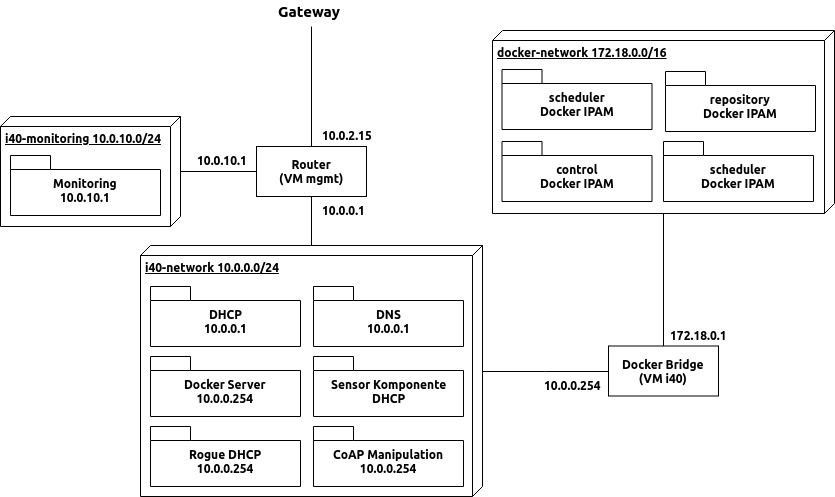
\includegraphics[width=12cm]{netzwerk}
  \caption{Netzwerkinfrastruktur} 
  \label{Konzept:Netzwerkkonzept}
\end{figure}

Die Kapselung und Sicherheit des Testsystems ist durch die Erweiterung um zusätzliche \ac{VM}s und Dienste weiterhin gegeben. Die Kommunikation mit dem Hostsystem und externen Netzen findet ausschließlich über die Netzwerkschnittstelle des Routers statt und dient der Installation und Konfiguration der Komponenten. Diese kann im Betrieb deaktiviert werden, um eine vollständige Isolation der Umgebung zu erzielen.

Durch die Konfigurationsmöglichkeiten der Hardware und des Netzwerks ist eine weitere Kapselung der Netzwerke mit Hilfe von \ac{VLAN} auf der Netzzugangssicht umsetzbar. Dies wird im Rahmen der Thesis jedoch aus zeitlichen Gründen nicht weiter bearbeitet.

\subsection{Industrienetzwerk}
Das Industrienetzwerk "`i40-network"' stellt den zentralen Bestandteil der Architektur dar. Dieses Netzwerk wird von den Diensten \ac{DHCP} und \ac{DNS} verwaltet und beinhaltet das Industrie 4.0 Produktionssystem und dessen Docker Sub-Architektur sowie die Sensor Komponente, welche Daten zum \ac{CoAP} Monitoring liefert. Der Netzwerkverkehr sowie die Verwaltung des Containernetzwerks wird vom Docker Dienst und dessen Netzwerkbrücke übernommen. Die Kommunikation mit dem Monitoringnetzwerk sowie mit externen Netzen wird mit Hilfe von \ac{IP} Forwarding und \ac{NAT} hergestellt. Der Rogue \ac{DHCP} Server befindet sich ebenfalls in diesem Netz und dient der Manipulation des für das Netzwerk \textit{authorativen} \ac{DHCP} Servers. Die Umsetzung dieses Netzwerks, der beinhalteten Dienste und der vollständigen Kontrolle über diese ist die Basis für die Durchführung der Anwendungsszenarien.

\subsection{Monitoring-Netzwerk}
Das Netzwerk "`i40-monitoring"' simuliert ein zusätzliches Netzwerk, welches Dienste zur Analyse und Überwachung der Komponenten im Netzwerk bereitstellen soll. Im beschriebenen Konzept besitzt das Monitoring-Netzwerk ausschließlich eine Komponente zur Überwachung der gesendeten Daten des im "`i40-network"' vorhandenen Sensors. Eine weitere Ausführung der Komponenten im Netzwerk hätte keinen Einfluss auf die gewählten Anwendungsszenarien (\autoref{Anwendungsszenarien:MitM} und \autoref{Anwendungsszenarien:Manipulation von ungesichertem Netzwerkverkehr}) gehabt, da die Kommunikation über ein Gateway der ausschlaggebende Faktor für die Integration des zusätzlichen Netzwerks war. Aus diesem Grund wurde auch kein \ac{DHCP} und \ac{DNS} für das Netzwerk konfiguriert. Die Adressvergabe verläuft statisch.

\subsection{Containernetzwerk}
Das Containernetzwerk beschreibt das grundlegende Testsystem und wird in \cite{Weber2018} beschrieben. Die bereitgestellten Container der Industrie 4.0 Umgebung werden durch den Docker Server verwaltet. Dieser übernimmt das \ac{IPAM} sowie den \ac{DNS}. Die Kommunikation zwischen den Containern sowie mit dem Hostsystem findet über eine Bridge\footnote{Eine Bridge verbindet zwei Segmente im Computernetz} statt. Diese Form der Netzwerkkommunikation ermöglicht es das Anwendungsszenario \autoref{Anwendungsszenarien:OPC UA Kommunikation} durchzuführen. Die Software-Bridge nimmt den gesamten Netzwerkverkehr entgegen und leitet ihn weiter. Somit ist es möglich diesen vom System, welches die Container verwaltet, zentral zu untersuchen.

\section{Bausteinsicht}
Die aus den Anwendungsszenarien (\autoref{Anwendungsszenarien}) hervorgehenden Anforderungen müssen durch die Komponenten im System umgesetzt werden. Hinzu kommt, dass die beschriebenen Netzwerke durch erforderlichen Dienste verwaltet werden müssen, um die Kommunikation der Komponenten zu gewährleisten. Die logische Darstellung der Verteilungssicht unterscheidet sich grundlegend von der Umsetzung der Komponenten in der Bausteinsicht. Die Virtualisierung der Maschinen erlaubt es mehrere Komponenten auf einem System zusammenzufassen und mit mehreren Netzwerkschnittstellen in verschiedenen Netzen auszustatten, um multiple Systeme darstellen zu können.

In \autoref{Konzept:Virtuelle Maschinen} werden die \ac{VM}s sowie deren Dienste und Schnittstellen in die Netzwerke dargestellt. Die Dienste \ac{DHCP}, \ac{DNS} im Netzwerk "`i40-network"' sowie die generellen Routingfunktionalitäten werden von der \ac{VM} "`mgmt"' bereitgestellt. Des Weiteren wird dort der \ac{CoAP} Server umgesetzt, welcher sich im Netzwerk "`i40-monitoring"' befindet. Die \ac{VM} "`i40"' beinhaltet die Komponenten zur Manipulation des Netzwerks sowie das Containernetzwerk. Der \ac{CoAP} Client des Netzwerk "`i40-network"' wird auf der \ac{VM} "`comp"' ausgeführt.

\begin{figure}[h]
  \centering
  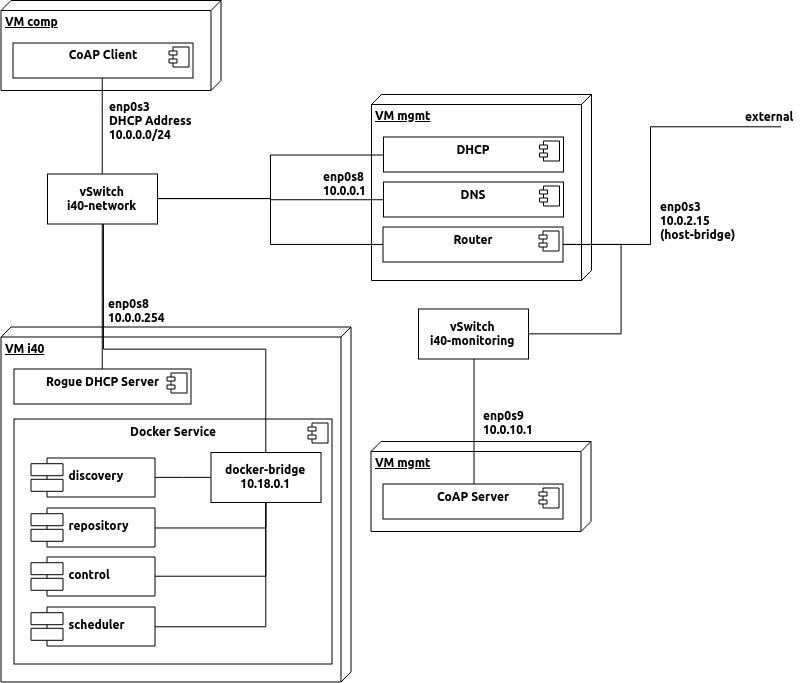
\includegraphics[width=12cm]{vm}
  \caption{Virtuelle Maschinen und Dienste} 
  \label{Konzept:Virtuelle Maschinen}
\end{figure}

\subsection{Router}
Die Routingfunktionalitäten werden auf der \ac{VM} "`mgmt"' umgesetzt. Die \ac{VM} besitzt in jedem Netzwerk ein Interface, welches als Schnittstelle dient und zur Weiterleitung der Pakete genutzt wird. Die \ac{VM} "`mgmt"' ist die einzige Komponente der Architektur, welche eine Verbindung zum Hostsystem besitzt. Die Weiterleitung der Pakete wird auf der Internetschicht des \ac{TCP}/\ac{IP} Referenzmodells mit Hilfe von \ac{IP}v4 Forwarding und \ac{NAT} umgesetzt. Durch das Routing zum Hostsystem ist eine Verbindung der anderen, gekapselten Maschinen sowie zukünftiger Maschinen für Installations- und Konfigurationszwecke in externe Netzwerke möglich. Um die Sicherheit des Netzwerkverkehrs sicherzustellen dürfen nur Pakete von Verbindungen, welche aus einem der internen Netze initiiert wurden weitergeleitet werden. \autoref{Konzept:Routerkomponente} stellt die Schnittstellen der Komponente dar.  

\begin{figure}[h]
  \centering
  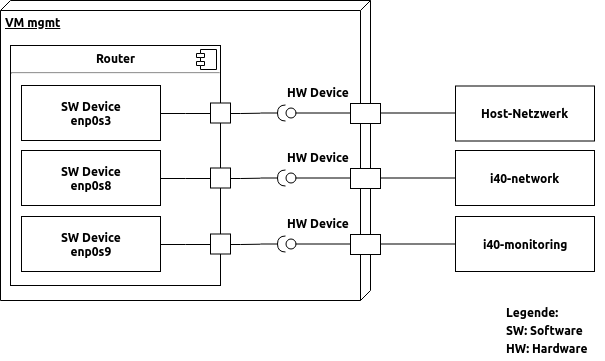
\includegraphics[width=12cm]{router}
  \caption{Routerkomponente} 
  \label{Konzept:Routerkomponente}
\end{figure}

\subsection{\ac{DHCP} Server/\ac{DNS} Server}
Die Dienste \ac{DHCP} und \ac{DNS} werden zusammen auf der \ac{VM} "`mgmt"' konfiguriert, stellen ihre Dienste im Netzwerk "`i40-network"' bereit, indem sie auf die zuständige Schnittstelle gebunden werden. Zur Umsetzung der Anwendungsszenarien \autoref{Anwendungsszenarien:MitM} und \autoref{Anwendungsszenarien:Manipulation von ungesichertem Netzwerkverkehr} liegt der Fokus der bereitzustellenden Funktionalität auf dem \ac{DHCP} Server. Dieser muss den weiteren Komponenten im Netzwerk beim \ac{DHCP} \textit{discover}, welcher über einen Broadcast\footnote{Eine Nachricht, die an alle Teilnehmer des Netzes gesendet und von diesen empfangen wird} durchgeführt wird, eine Netzwerkkonfiguration bereitstellen. Dabei ist die Vergabe eines Standardgateways für die spätere Durchführung des \ac{MitM} Anwendungsszenario essentiell. Das \ac{IPAM} sowie die Konfiguration des \ac{DNS} und dessen dynamische Zonenaktualisierungen spielen bei der Umsetzung des Angriffs nur eine nebensächliche Rolle. Sie werden jedoch trotzdem umgesetzt, da die Konfiguration des \ac{IPAM} und der \textit{address range} der \ac{DHCP} \textit{leases} eine Möglichkeit gibt den Wechsel des \ac{DHCP} Servers zu Lehrzwecken visualisieren zu können. Die Bereitstellung eines mit dem \ac{DHCP} Server kompatiblen \ac{DNS} Servers vereinfacht durch die Namensauflösung die Verwaltung der virtuellen Maschinen in der Testumgebung und ermöglicht eine skalierbare Erweiterung des Systems. Die Verwaltung eines separaten \ac{DNS} Servers ermöglicht die Umsetzung weiterer Anwendungsszenarien und die Analyse des Sicherheitsmechanismus \ac{DNSSEC} am Testsystem. Diese Anwendungsmöglichkeiten sind kein Bestandteil der Thesis und werden im weiteren Verlauf nicht weiter erläutert. Sie bieten jedoch Ansatzmöglichkeiten für zusätzliche Erweiterungen am System und werden in \autoref{Fazit} näher beschrieben.

\autoref{Konzept:DHCP und DNS Server} zeigt die Komponenten \ac{DHCP} Server und \ac{DNS} Server und die genutzten Schnittstellen in Bezug auf das Gesamtsystem. Beide Dienste werden auf das Netzwerkinterface des Netzwerks "`i40-network"' gebunden. Somit werden die Dienste ausschließlich im beschriebenen Netzwerk bereitgestellt.

\begin{figure}[h]
  \centering
  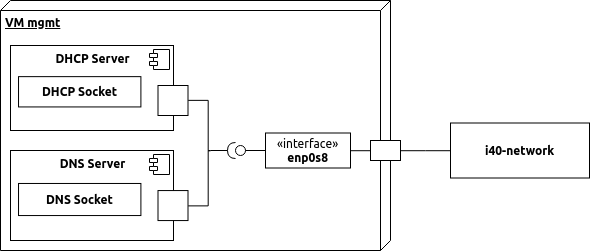
\includegraphics[width=12cm]{dhcpdns}
  \caption{DHCP und DNS Server} 
  \label{Konzept:DHCP und DNS Server}
\end{figure}

\subsection{\ac{CoAP} Client/\ac{CoAP} Server}
Die Komponenten \ac{CoAP} Client und \ac{CoAP} Server dienen der Erweiterung des Testsystems um ein weiteres \ac{IIoT} Protokoll zur Darstellung des in \autoref{Anwendungsszenarien:Manipulation von ungesichertem Netzwerkverkehr} beschriebenen Szenarios. Die Komponenten simulieren einen Temperatursensor sowie ein Monitoringsystem, welches ein Webinterface zur Darstellung der gemessenen Temperatur besitzt. Der \ac{CoAP} Client wird auf der \ac{VM} "`comp"' realisiert und befindet sich im Netzwerk "`i40-network"'. Er sendet die gemessenen Daten zum zuständigen \ac{CoAP} Server im Netzwerk "`i40-monitoring"'. Der \ac{CoAP} Server wird, da er den einzigen Dienst in diesem Netzwerk darstellt, auf der \ac{VM} "`mgmt"' bereitgestellt. Die \ac{VM} "`mgmt"' besitzt bereits ein Interface im Netzwerk "`i40-monitoring"'. Der Dienst kann auf die Adresse der Schnittstelle gebunden werden. Es muss keine weitere \ac{VM} zum Netzwerk hinzugefügt werden.

\autoref{Konzept:CoAP Client} und \autoref{Konzept:CoAP Server} visualisieren die Bestandteile der betroffenen Komponenten, deren bereitgestellte Dienste und die genutzten Schnittstellen.

\begin{figure}[h]
  \centering
  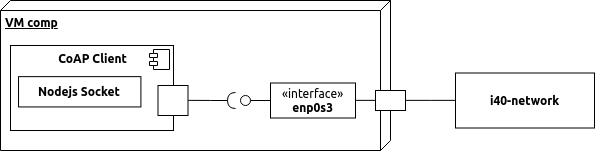
\includegraphics[width=12cm]{coapClient}
  \caption{CoAP Client} 
  \label{Konzept:CoAP Client}
\end{figure}

\begin{figure}[h]
  \centering
  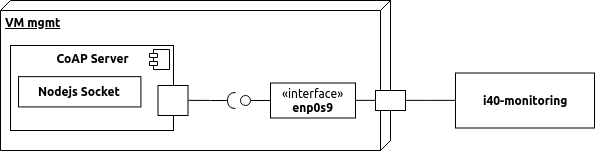
\includegraphics[width=12cm]{coapServer}
  \caption{CoAP Server} 
  \label{Konzept:CoAP Server}
\end{figure}

\subsection{Rogue \ac{DHCP} Server}
Die Bereitstellung des Rogue \ac{DHCP} Servers findet auf der bestehenden \ac{VM} "`i40"' statt. Die bestehende virtuelle Maschine stellt bereits Tools zu Analyse der Netzwerkkommunikation für das Dockernetzwerk bereit. Eine Erweiterung dieses Systems ermöglicht es die bereitgestellten Anwendungen zur Analyse in den Anwendungsszenarien des Netzwerks der \ac{VM}s ebenfalls zu nutzen. Dies wird durch die Trennung der Netzwerkschnittstellen ermöglicht. Die Analyse der Pakete findet fortan auf der Schnittstelle "`enp0s8"' der Docker Netzwerkbrücke statt. Um die Netzwerkpakete der anderen Teilnehmer über die Schnittstelle der \ac{VM} zu leiten, muss die Maschine selbst als Gateway für die Kommunikation zwischen den Netzen genutzt werden. Der Rogue \ac{DHCP} Server ermöglicht die Änderung des Standardgateways bei Erneuerung des \ac{DHCP} \textit{lease} der Client und kann somit den Verkehr auf das lokale System umleiten. \autoref{rogueDhcp} zeigt die Eingliederung des Dienstes in das vorhandene System. Der Dienst muss im Netzwerk "`i40-network"' agieren und wird somit auf das Interface "`enp0s8"' gebunden.

\begin{figure}[h]
  \centering
  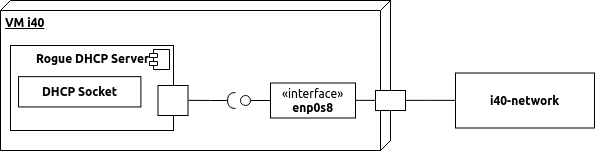
\includegraphics[width=12cm]{rogueDhcp}
  \caption{Rogue DHCP Server} 
  \label{Konzept:Rogue DHCP Server}
\end{figure}

\subsection{\ac{CoAP} Manipulationssystem}
Das \ac{CoAP} Manipulationssystem wird genutzt, um das \ac{CoAP} Monitoringsystem durch falsche bzw. unzulässige Netzwerkpakete zu beeinflussen. Es wird ebenfalls auf der \ac{VM} "`i40"' bereitgestellt. Dies ermöglicht weiterhin die zentrale Verwaltung des Systems und die Durchführung der Anwendungsszenarien. Eine Bereitstellung des Manipulationsdienstes auf dem gleichen System wie der Rogue \ac{DHCP} Server und die Anwendungen zur Netzwerkanalyse ist sinnvoll, da die Umleitung der Netzwerkpakete durch den Rogue \ac{DHCP} Server und die anschließende Analyse des Verkehrs die Grundlage für die Manipulation des Monitoringsystems darstellt und voneinander abhängig ist.

Das \ac{CoAP} Manipulationssystem versendet Netzwerkpakete mit gefälschten Daten zum \ac{CoAP} Monitoringsystem. Diese werden über die Netzwerkschnittstelle "`enp0s8"' in das "`i40-network"' versandt. Die Verbindung in das Netzwerk "`i40-monitoring"' wird über die Routingfunktionalitäten der \ac{VM} "`mgmt"' bereitgestellt. \autoref{Konzept:CoAP Manipulationssystem} beschreibt den Aufbau der Komponente.

\begin{figure}[h]
  \centering
  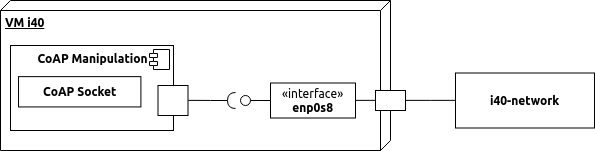
\includegraphics[width=12cm]{coapManipulation}
  \caption{CoAP Manipulationssystem} 
  \label{Konzept:CoAP Manipulationssystem}
\end{figure}

\subsection{Docker Service}
An der Netzwerkkonfiguration sowie am Docker Service der \ac{VM} "`i40"' wurden keine Änderungen vorgenommen. Die genutzte Konfiguration des Dienstes ist in \cite{Weber2018} erläutert. Eine Integration der neuen Komponenten als zusätzliche Container im bestehenden Netzwerk war nicht möglich, da dies die Analyse des Netzwerks durch die Netzwerkimplementierung der Software Docker verfälscht bzw. verhindert. Eine genaue Beschreibung der Beschränkungen, welche bei der Umsetzung des Systems zum Tragen kamen, wird in \autoref{Konzept:Softwarebeschränkungen} durchgeführt.

\section{Laufzeitsicht}
Die Laufzeitsicht dient der Darstellung der Kommunikation zwischen den einzelnen Komponenten zur Bereitstellung einer Gesamtfunktionalität. In diesem Abschnitt werden die essentiellen Abläufe des Systems, welche die Netzwerkkommunikation und -konfiguration zwischen den Komponenten bereitstellen, in Anlehnung an \ac{UML}-Sequenzdiagramme dargestellt.

\subsection{Routing}
Um eine Verbindung zwischen den Netzwerken "`i40-network"' und "`i40-monitoring"' herzustellen und die Kommunikation der \ac{CoAP} Komponenten im Netzwerk zu gewährleisten, muss die \ac{VM} "`mgmt"', welche als einziges System eine Schnittstelle in beiden Netzwerken bereitstellt, Routingfunktionalitäten übernehmen. Dabei müssen eine Weiterleitung der Pakete zwischen den Netzwerkschnittstellen der \ac{VM} stattfinden.

\subsection{\ac{DHCP}}
Im Netzwerk "`i40-network"' werden die Dienste \ac{DHCP} und \ac{DNS} zur dynamischen Konfiguration und Namensauflösung der Hosts genutzt. \autoref{Konzept:Dynamische Hostkonfiguration mit DHCP und DNS} zeigt die Konfiguration eines Hosts beim Bezug der Netzwerkkonfiguration im "`i40-network"' mit Hilfe des zuständigen \ac{DHCP} Servers. Die Netzwerknachrichten der \ac{DHCP} Konfiguration werden, da der Client zum Zeitpunkt der dynamischen Konfiguration noch keine \ac{IP} Adresse im Netzwerk besitzt, über den Broadcast im Netzwerk versandt. Die Pakete werden ausschließlich von \ac{DHCP} Servern angenommen und verarbeitet, weitere Clients im Netzwerk verwerfen die Pakete. Im Sequenzdiagramm ist, um die Übersichtlichkeit zu gewährleisten, nur die Kommunikation zwischen den aktiv beteiligten Komponenten während der dynamischen Konfiguration des Hosts dargestellt.

Um vollständige Funktionalität des Clients im Netzwerk bereitzustellen, werden \ac{IP} Adresse, Netzwerkmaske, \ac{DNS} sowie ein Gateway zur Verbindung in andere Netze benötigt. Nach dem \ac{DHCP} Discover des Clients bietet der \ac{DHCP} Server mit Hilfe des \ac{DHCP} Offer Netzwerkkonfigurationen für den Client an. Dieser bestätigt die Konfiguration mit einem \ac{DHCP} Request. Ist die vom Server angebotene Konfiguration gültig und die \ac{IP} Adresse weiterhin frei, wird vom Server ein \ac{DHCP} Ack gesendet, um die Konfiguration zu bestätigen.

\ac{DNS} und \ac{DHCP} arbeiten im Testsystem zusammen. Der \ac{DHCP} Server muss den \ac{DNS} Server über neue Clients im Netzwerk informieren, um eine Namensauflösung dieser bereitstellen zu können. Die Authentifizierung zur Kommunikation und Aktualisierung der \ac{DNS} Zonen geschieht mit Hilfe eines symmetrischen Schlüssels. Beide Komponenten müssen diesen Schlüssel besitzen, um sich beim anderen Dienst zu authentifizieren. Die dynamische Aktualisierung einer \ac{DNS} Zone wird ebenfalls in \autoref{Konzept:Dynamische Hostkonfiguration mit DHCP und DNS} beschrieben.

\begin{figure}[h]
  \centering
  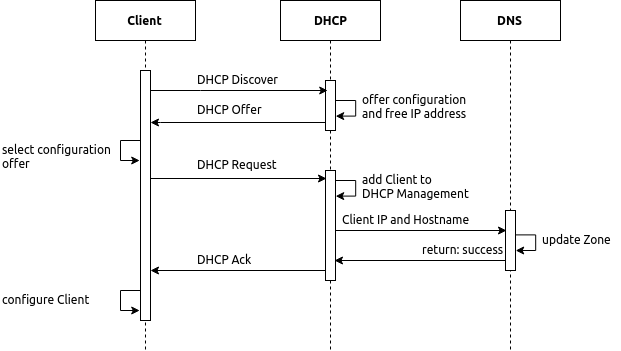
\includegraphics[width=12cm]{dhcpdnsseq}
  \caption{Dynamische Hostkonfiguration mit DHCP und DNS} 
  \label{Konzept:Dynamische Hostkonfiguration mit DHCP und DNS}
\end{figure}

\subsection{\ac{DNS}}
Die Namensauflösung der internen Adressen findet direkt auf dem \ac{DNS} Server statt. Bei einem \ac{DNS} Request werden die lokalen Zonendateien durchsucht und in der Answer Section der \ac{DNS} Response die gewünschten \ac{RR} bereitgestellt. Das interne Netzwerk "`i40-network"' besitzt eine Zone auf dem Nameserver. Dort müssen alle statischen Adressen zur Namensauflösung eingetragen werden. Die dynamischen Adressen werden ebenfalls in dieser Zone temporär hinterlegt. Um eine Namensauflösung in externe Netze zu gewährleisten, muss der \ac{DNS} Server weitere Nameserver kennen, um Domainnamen, welche nicht in der Datenbank des lokalen Servers vorhanden sind, aufzulösen. Das \ac{DNS} System nutzt Rekursion oder Iteration, um den \textit{authorativen} Server im Netzwerk zu bestimmen und die Namensauflösung bereitzustellen. Der Ablauf der Namensauflösung wird vom zuständigen Nameserver bestimmt. \autoref{Konzept:Rekursive DNS Namensauflösung} stellt den Ablauf der rekursiven Namensauflösung einer externen \ac{DNS} Zone vereinfacht dar. Der lokale \ac{DNS} Server arbeitet als \ac{DNS}-Forwarder. Er leitet die Anfrage zur unbekannten Zone an einen externen \ac{DNS} weiter, welcher die Adresse auflöst und dem internen Nameserver das Ergebnis mitteilt. Die Rekursion der Befragung weiterer \ac{DNS} Server findet solange statt, bis ein für die Domain zuständiger Nameserver gefunden wurde, welcher die Adresse auflöst. Bei der iterativen Namensauflösung sendet der \ac{DNS} Server dem Client die Adresse des \textit{authorativen} \ac{DNS} Servers zu. Dieser führt dann einen erneuten \ac{DNS} Query bei diesem Server durch. Der Ablauf der iterativen Namensauflösung wird in \autoref{Konzept:Iterative DNS Namensauflösung} dargestellt.

Die genutzte Form der Namensauflösung hat auf die Umsetzung des Konzepts keinen Einfluss. Um eine Namensauflösung in externe Netze bereitzustellen muss der \ac{DNS} Server lediglich eine erreichbare \ac{DNS} Forward-Adresse besitzen.  

\begin{figure}[h]
  \centering
  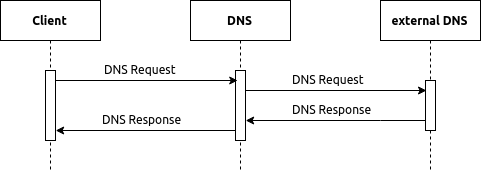
\includegraphics[width=12cm]{dnsrekseq}
  \caption{Rekursive DNS Namensauflösung} 
  \label{Konzept:Rekursive DNS Namensauflösung}
\end{figure}

\begin{figure}[h]
  \centering
  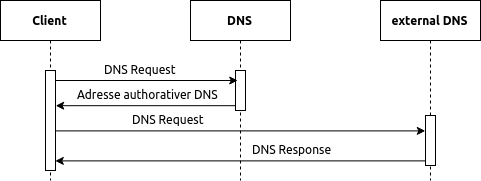
\includegraphics[width=12cm]{dnsitseq}
  \caption{Iterative DNS Namensauflösung} 
  \label{Konzept:Iterative DNS Namensauflösung}
\end{figure}

\subsection{Kommunikation CoAP Client und Server}
Das Zusammenspiel der bisher beschriebenen Komponenten wird für die Kommunikation zwischen \ac{CoAP} Client und \ac{CoAP} Server benötigt. Im in \autoref{Anwendungsszenarien:Manipulation von ungesichertem Netzwerkverkehr} beschriebenen Anwendungsszenario findet zwischen den Komponenten ausschließlich eine unidirektionale\footnote{Eine unidirektionale Verbindung findet nur in eine Richtung an einen oder mehrere Empfänger statt} Kommunikation vom Client zum Server statt. \autoref{Konzept:CoAP Client und Server} zeigt die Netzwerkkonfiguration des Clients und die genutzten Komponenten bei der Übermittlung einer Nachricht vom Client zum Server und steht beispielhaft für die Kommunikation aller Komponenten im Netzwerk. Um die Übersichtlichkeit der Darstellung zu erhalten, findet nur noch eine einfache Beschreibung der Initialisierung des Clients statt. Diese wurde bereits in \autoref{Konzept:Dynamische Hostkonfiguration mit DHCP und DNS} beschrieben. Die Kommunikation zwischen \ac{CoAP} Client und \ac{DHCP} findet im Netzwerk "`i40-network"' statt. Die Kommunikation zwischen dem Client und Server erfordert die Nutzung eines Routers, da sich die Serverkomponente im Netzwerk "`i40-monitoring"' befindet. Die Struktur der Netzwerkkommunikation gilt für alle Komponenten des Netzwerks "`i40-network"'.

\begin{figure}[h]
  \centering
  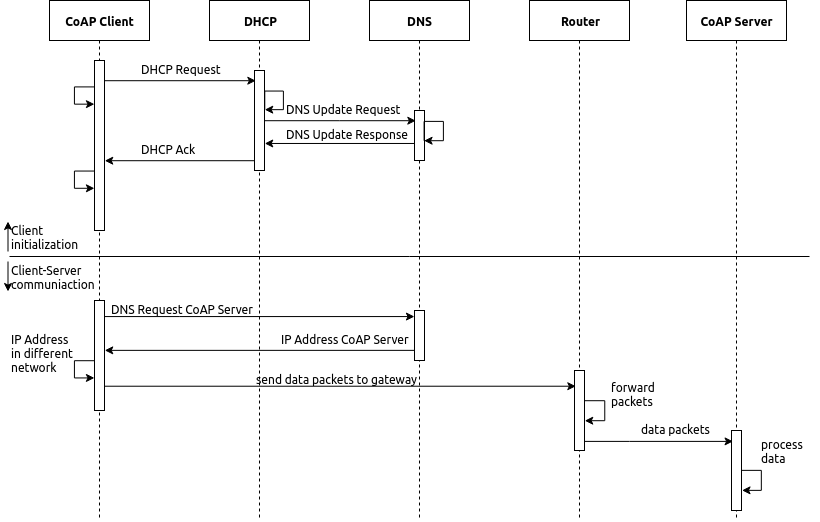
\includegraphics[width=12cm]{coapseq}
  \caption{Initialisierung von CoAP Client und Kommunikation zwischen CoAP Client und CoAP Server} 
  \label{Konzept:CoAP Client und Server}
\end{figure}

\subsection{Manipulation des Netzwerkverkehrs}
Durch die Aktivierung der Rogue \ac{DHCP} Komponente auf der \ac{VM} "`i40"' wird ein zweiter \ac{DHCP} Server im Netzwerk aktiviert. Komponenten, welche über einen \ac{DHCP} Discover den für das Netzwerk zuständigen \ac{DHCP} Server kontaktieren möchten, können nun auch eine Antwort des Rogue \ac{DHCP} Servers erhalten. Dieser stellt eine \ac{DHCP} Konfiguration mit sich selbst als Gateway bereit. Trifft der \ac{DHCP} Offer des Rogue \ac{DHCP} Servers vor dem \ac{DHCP} Offer des eigentlichen \ac{DHCP} Servers beim Client ein, sendet dieser den gesamten Netzwerktraffic, welcher für andere Netze bestimmt ist über den neuen \ac{DHCP} Server. Um die Netzwerkkommunikation der Systeme, welche den Rogue \ac{DHCP} Server als Gateway nutzen weiterhin bereitzustellen, muss dieser die Pakete wieder zum ursprünglichen Router weiterleiten. Der Ablauf der Kommunikation wird in \autoref{Konzept:Umleitung der Netzwerkkommunikation durch Manipulation des Gateways} vereinfacht beschrieben. \ac{DHCP} Nachrichten werden nicht gerichtet an Systeme gesendet, diese werden über den Broadcast des Netzwerks kommuniziert. Die \ac{DNS} Namensauflösung wurde in der Darstellung nicht aufgeführt, da sie zur Umleitung der Netzwerkpakete in diesem Beispiel keinen Beitrag leistet.

\begin{figure}[h]
  \centering
  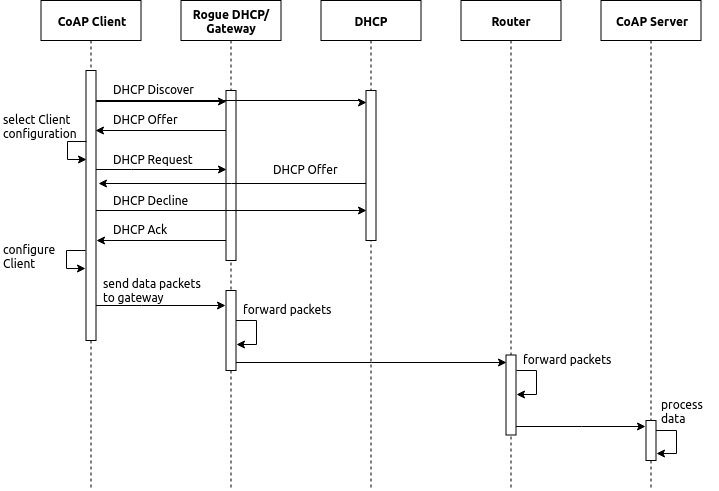
\includegraphics[width=12cm]{coapMani}
  \caption{Umleitung der Netzwerkkommunikation durch Manipulation des Gateways} 
  \label{Konzept:Umleitung der Netzwerkkommunikation durch Manipulation des Gateways}
\end{figure}

\section{Anpassungen}
\label{Konzept:Anpassungen}
Im Laufe der Entwicklung des Konzepts mussten immer wieder Anpassungen vorgenommen werden. Diese bezogen sich auf die Umsetzbarkeit des Konzepts in Bezug zu dem im Testsystem bisher verwendeten Softwarestack. 

Ursprünglich wurde die Erweiterung des Testsystems um zusätzliche Docker Container, welche die aus den in \autoref{Anwendungsszenarien} beschriebenen Anwendungsszenarien hervorgehenden Anforderungen sowie die benötigte Netzwerkinfrastruktur umsetzen, geplant. Dies war nicht möglich, da die Containervirtualisierung kein vollständiges System inklusive Hardwarekomponenten simuliert, sondern lediglich ein isoliertes Gastsystem darstellt, welches den Kernel und die Komponenten des Hostsystems nutzt. Die Netzwerkimplementierung der genutzten Software Docker stellt vier Netzwerktreiber\footnote{Docker Netzwerktreiber - https://docs.docker.com/network/} zur Kommunikation der Container mit anderen Komponenten bereit. Jeder dieser Treiber stellt ein eigenes, statisches \ac{IPAM} mit Hilfe des Docker Service bereit. Der Treiber \textit{macvlan} simuliert zwar eine physikalische Schnittstelle der Container mit Hilfe einer \ac{MAC} Adresse, jedoch übernimmt der Docker Service weiterhin das \ac{IPAM}. Die Adressvergabe und Netzwerkkonfiguration ist somit weiterhin nur statisch beim Start der Container möglich. 

Eine Alternative würde die Nutzung von Pipeworks\footnote{Pipeworks - https://github.com/jpetazzo/pipework} darstellen. Die Software ermöglicht es die Container zu einem logischen, physikalischen Interface zu verbinden, indem sie im Container einen zusätzlichen Netzwerkadapter bereitstellt. Somit könnte die externe Verwaltung der Docker Netzwerkschnittstellen über einen \ac{DHCP} Server bereitgestellt werden. Die Software stellt keine solide Implementierung bereit und rät dazu, wenn möglich, auf die offiziellen Implementierungen von Docker zurückzugreifen. Mit der Erweiterung des Systems um zusätzliche Softwareimplementierungen können weitere Nebeneffekte oder Probleme bei der Umsetzung der Anwendungsszenarien aufgrund von Softwarebeschränkungen entstehen.

Da keiner der beschriebenen Ansätze eine zufriedenstellende Lösung zur Umsetzung der Anwendungsszenarien bereitstellt, wurde die Erweiterung des Systems und die Darstellung verschiedener Netzwerkkomponenten und deren Kommunikation mit Hilfe von \ac{VM}s realisiert. \ac{VM}s werden in Industrie 4.0 Netzwerken weitreichend und produktiv genutzt. Sie können die Infrastruktur repräsentieren und bieten auch für die Zukunft eine stabile Grundlage zur Integration weiterer Dienste im Testsystem. Sie stellen umfangreiche Konfigurationsmöglichkeiten für die virtualisierte Hardware der Clients sowie das Netzwerk bereit.